```latex \documentclass[12pt]{article} \usepackage[margin=1in]{geometry} \usepackage{graphicx} \usepackage{booktabs} \usepackage{amsmath}
 \title{The Effect of Paid Search Advertising on Revenue: \\ A Replication of the eBay Natural Experiment} \author{Your Name} \date{\today} \begin{document} \maketitle \section{Introduction} This paper studies the causal effect of paid search advertising on eBay’s revenue. Firms spend billions of dollars each year on search engine marketing (SEM),
 yet measuring its true impact is difficult because advertising exposure is typically correlated with consumer demand. The central research question is whether paid search advertising meaningfully increases revenue for an established brand such as eBay. To answer this question, we replicate a natural experiment in which eBay temporarily turned off paid search advertising in selected markets.
 Using a difference-in-differences (DID) framework, we compare changes in revenue between treatment and control regions before and after advertising was suspended. \section{Experimental Setting} Blake, Nosko, and Tadelis (2014) persuaded eBay to stop bidding on Google AdWords in a subset of U.S. designated market areas (DMAs). Beginning on May 22, 2012, paid search advertising was turned off in 65 of the 210 DMAs for an eight-week period. These DMAs form the treatment group (search\_stays\_on = 0),
 while the remaining markets continued running paid search ads and serve as the control group (search\_stays\_on = 1). Importantly, this was not a fully randomized experiment. The largest DMAs were excluded from treatment, meaning that treatment and control markets differ in baseline revenue levels. Control DMAs tend to have higher average revenue because they include the largest metropolitan areas.
 As a result, a simple comparison of average revenue between groups would be biased. This motivates the use of a difference-in-differences approach, which focuses on changes over time within each group rather than level differences across groups. 
\section{Data and Figures} The dataset contains daily revenue data for 210 DMAs from April through July 2012. Key variables include the date, DMA identifier, treatment status, treatment period indicator, and daily revenue. The pre-treatment period runs from April 1 to May 21, 2012, and the post-treatment period begins on May 22, 2012. 
\begin{figure}[h] \centering 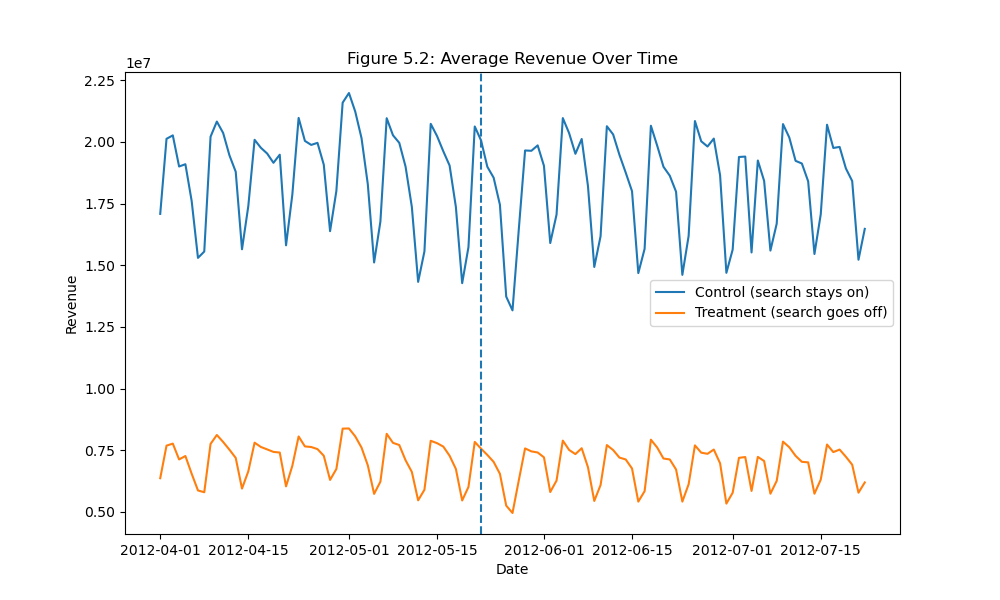
\includegraphics[width=0.85\textwidth]{../output/figures/figure_5_2.png} \caption{Average revenue for treatment and control DMAs over time. The dashed line marks May 22, 2012, when SEM was turned off for the treatment group.} \label{fig:revenue} \end{figure} 
Figure \ref{fig:revenue} plots average daily revenue for treatment and control DMAs over time. The control group consistently exhibits higher average revenue, reflecting the exclusion of the largest DMAs from treatment. Both groups display similar weekly oscillation patterns, suggesting common seasonal demand fluctuations.
 Visually, it is difficult to detect a clear divergence in revenue after May 22 at this scale. \begin{figure}[h] \centering 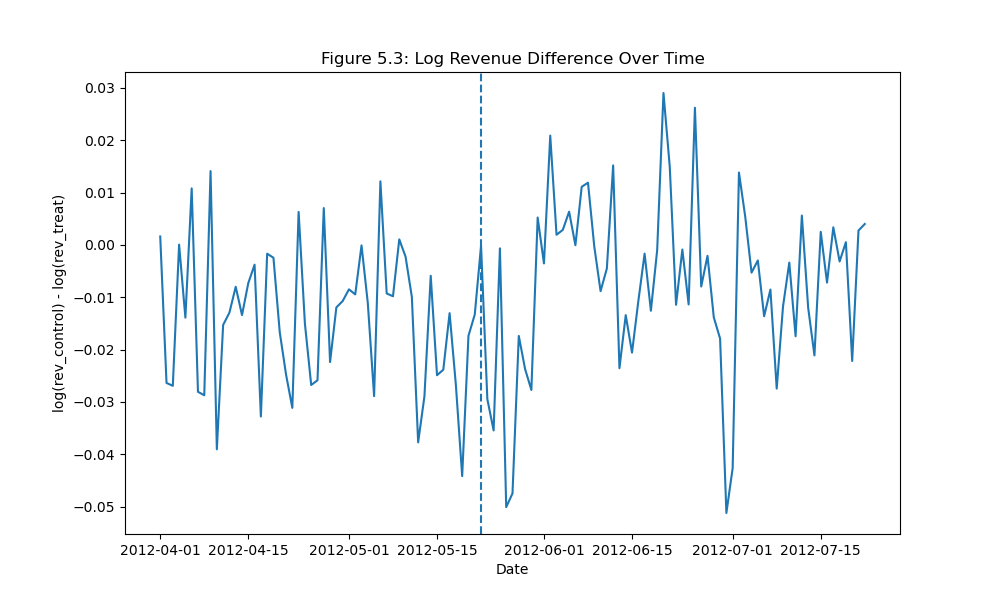
\includegraphics[width=0.85\textwidth]{../output/figures/figure_5_3.png} \caption{Log-scale average revenue difference between control and treatment groups over time. The gap appears to increase after May 22.} \label{fig:logdiff} \end{figure} 
Figure \ref{fig:logdiff} shows the log difference (or log ratio) of average revenue between control and treatment DMAs over time. Prior to May 22, the log gap fluctuates around a relatively stable level. After advertising is turned off in the treatment group, the gap appears to increase slightly. This visual pattern suggests a potential negative effect of removing paid search, motivating a formal DID estimation. 
\section{Results} \input{../output/tables/did_table.tex} The difference-in-differences estimate of the treatment effect is $\hat{\gamma} = -0.0066$ in log scale. Exponentiating this estimate yields $\exp(-0.0066) = 0.9934$, implying that turning off paid search reduced revenue by approximately 0.66 percent in treated DMAs. The estimated 95\% confidence interval in log scale is $[-0.0175, 0.0043]$, which corresponds to a levels interval of approximately $[0.9827, 1.0043]$. Because the confidence interval includes zero (or one in levels), the effect is not statistically significant at the 5 percent level. Economically, the estimated impact is very small in magnitude. This suggests that for a well-known brand like eBay, most consumers may find the platform through organic search results rather than paid advertisements. The findings therefore replicate the main conclusion of Blake, Nosko, and Tadelis (2014): paid search advertising had little incremental effect on revenue for eBay during this experiment. \section{Conclusion} Using a difference-in-differences framework, this paper replicates the eBay paid search experiment and finds a small, statistically insignificant effect of paid search advertising on revenue. The point estimate suggests a revenue decline of less than one percent when paid search was turned off, and the confidence interval includes zero. While the analysis relies on scaled revenue data and a simple DID specification without additional controls, the results are consistent with the original study’s conclusion that paid search may provide limited incremental value for established brands. These findings highlight the importance of causal identification when measuring marketing return on investment. \begin{thebibliography}{9} \bibitem{blake2014} Blake, T., C. Nosko, and S. Tadelis (2014). ``Consumer Heterogeneity and Paid Search Effectiveness: A Large-Scale Field Experiment.'' \textit{Econometrica}, 83(1): 155--174. \bibitem{taddy2019} Taddy, M. (2019). \textit{Business Data Science}. McGraw-Hill, Chapter 5. \end{thebibliography} \end{document} ```
